\RequirePackage[hyphens]{url} %Brechen von urls nach spiegelstrichen

\documentclass[a4paper,12pt]{article}
\usepackage[left= 2.5cm, right = 2.5cm, bottom = 4cm]{geometry}

\usepackage[british]{babel} % ngerman
\usepackage[scaled]{helvet} % use helvetica font
\usepackage[T1]{fontenc}
\usepackage[utf8]{inputenc}
\usepackage{float} %big H

\usepackage[pdfusetitle]{hyperref}
\hypersetup{ %https://en.wikibooks.org/wiki/LaTeX/Hyperlinks#Customization
    colorlinks = false, 
    hidelinks,
    breaklinks, %line breaking in a long hyperlink
    urlcolor=green, % farbe von \url
    linkcolor =green, %Farbe von \ref
    citecolor =green %Farbe von \cite
}

%Graphikpaket mit Datenpfad
\usepackage{graphicx}
\graphicspath{ {image/} }
\usepackage{caption} %https://en.wikibooks.org/wiki/LaTeX/Floats,_Figures_and_Captions
\usepackage{subcaption} %mehrere Bilder mit Untercaptions
\usepackage{wrapfig}

%Literaturverzeichnis
\usepackage{csquotes}
\usepackage{comment}
\usepackage[ % https://www.overleaf.com/learn/latex/Bibliography_management_with_biblatex#Reference_guide
    backend=biber, % biber backend
    natbib=true, % customising citations
    % sorting=nty, % sort name, title, year
    style=numeric % alphabetic, numeric
]{biblatex}
\addbibresource{references.bib}

%Nicht einrücken nach Absatz
\setlength{\parindent}{0pt}

% Set global margin for indents
\usepackage{enumitem}
\setlist{leftmargin=1cm}

%%Zeilenabstand
\usepackage[onehalfspacing]{setspace} %singlespacing. onehalf-, double-

%% zusätzliche Schriftzeichen der American Mathematical Society
\usepackage{amsfonts}
\usepackage{amsmath, bm}
\usepackage{amssymb}

% ============= First Page edits =============
\title{Computer Vision Projects: \\
Document Scanner}
\author{Anton Gres}

\date{3rd Mai 2021}

% needed to set font correctly for the whole document 
\renewcommand\familydefault{\sfdefault} 

\begin{document}

\maketitle
\thispagestyle{empty} %erzwingen von leerer Nummerierung

\vspace{1cm}

\tableofcontents %Inhaltsverzeichnis
\newpage

%\listoffigures %Abbildungsverzeichnis
%\newpage

\section{Objective}

The aim of this project is to develop an application which creates an undistorted image from a distorted image. This means that the distorted image with its non-straight edges should be transformed into an undistorted image, where the non-straight edges are straightened.\\ 

Distorted images are naturally generated by the camera because of its lens properties. It cannot be assumed that even cameras of the same model have the exact same lens properties. That's why it is important to calibrate every camera for its intrinsic matrix, which can be used to undistort the images. \cite{cv}\\

To achieve this goal in this project, recordings have been provided as a source which show an 8x8 chessboard. In these, the chessboard is placed by a person in different positions and at different angles to the camera. These frames in the recordings are the basis for the camera calibration.\\
\vspace{-2mm}
\begin{wrapfigure}{L}{0.57\textwidth}
    \centering
     \captionsetup{justification=centering}
     \vspace{-4mm}
     \begin{minipage}[b]{0.55\textwidth}
         \centering
         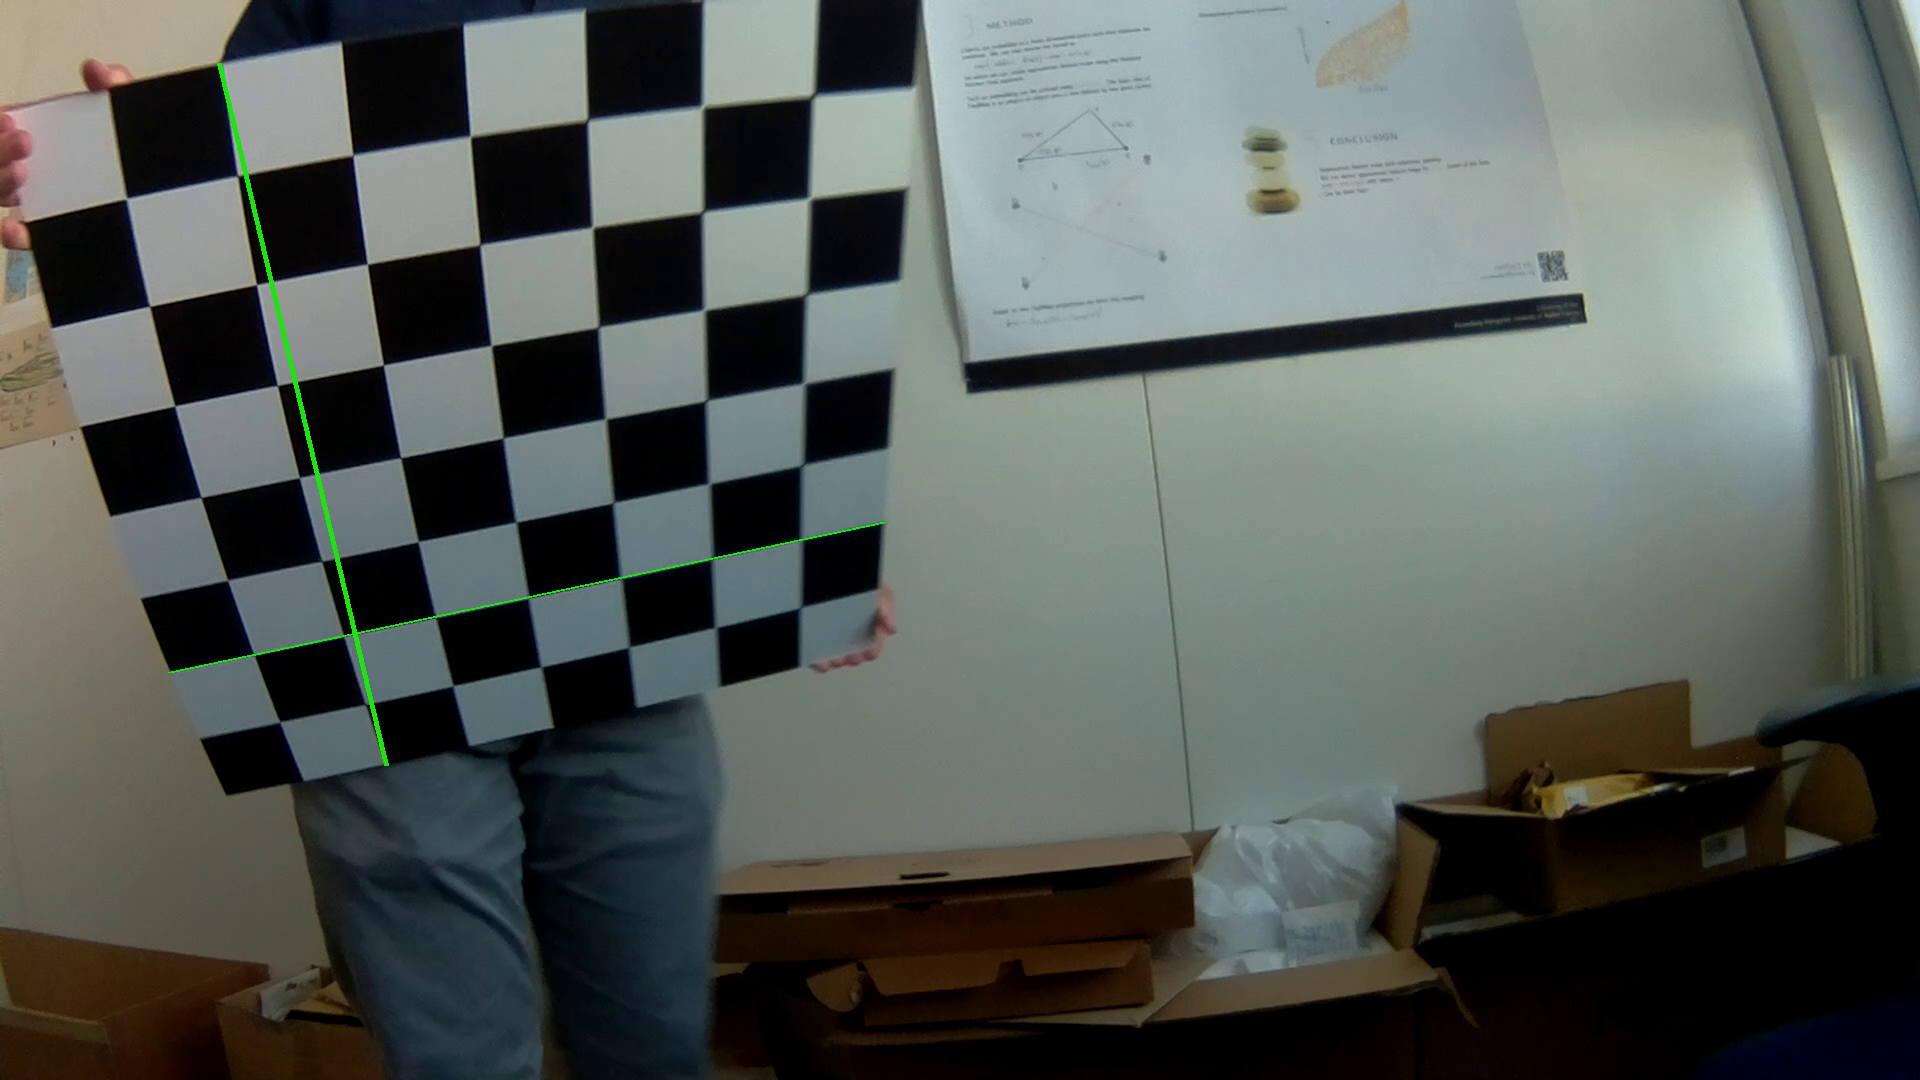
\includegraphics[width=\textwidth]{image/1/og.png}
         \caption{Distorted (original) frame from the source recording}
         \label{fig:og_frame}\par
         \vspace{6mm}
         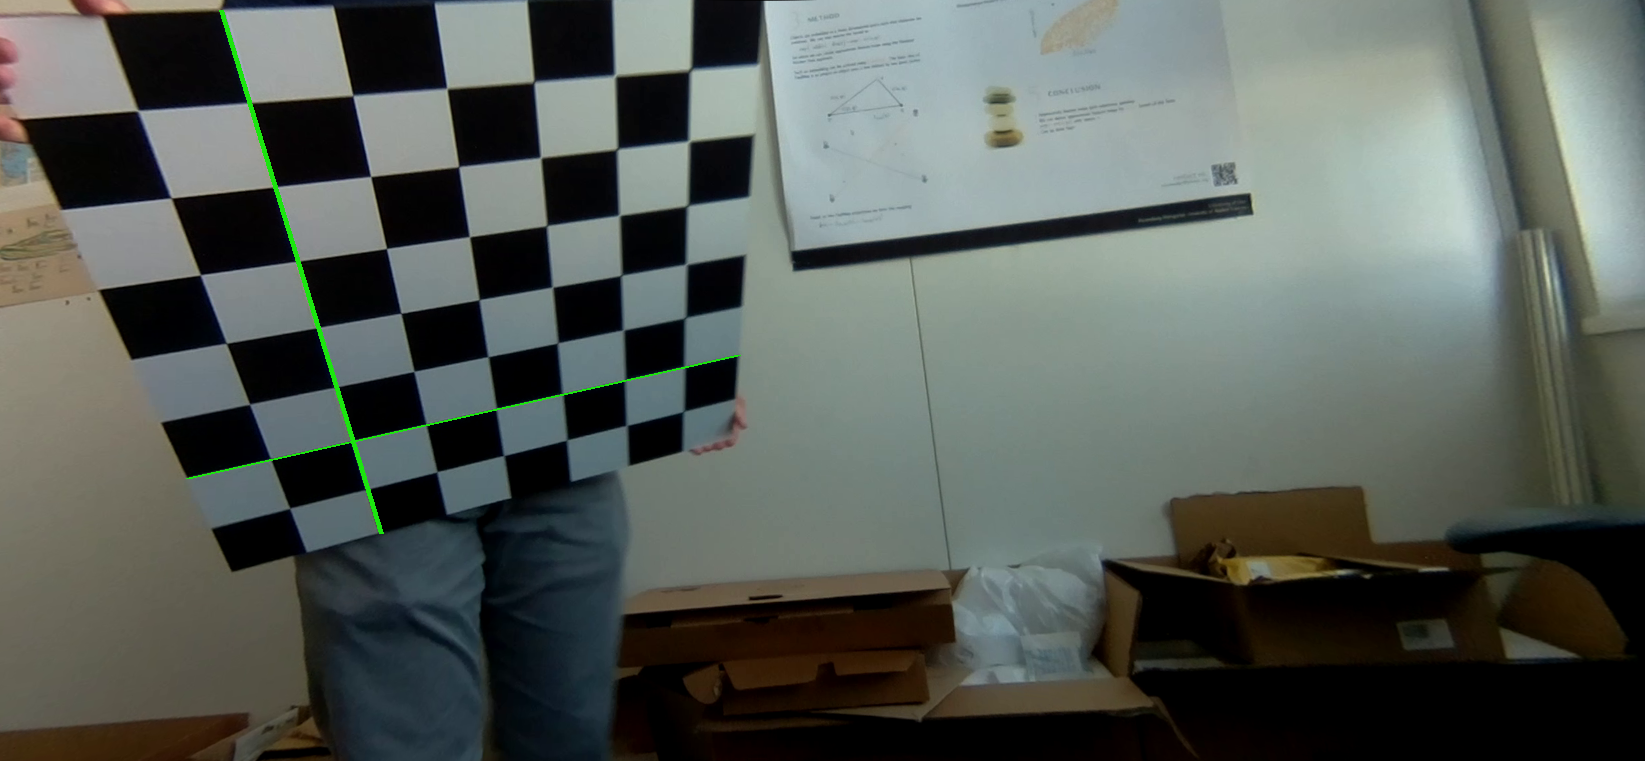
\includegraphics[width=\textwidth]{image/1/undist.png}
         \caption{Undistorted frame}
         \label{fig:dst_frame}
     \end{minipage}
     \hfill
     \vspace{-9mm}
\end{wrapfigure}

Figure \ref{fig:og_frame} shows an example frame of the recording and figure \ref{fig:dst_frame} the undistorted image of the distorted frame. The straight green line should serve as a reference to compare the non-straight edges to the straight edges of the checkerboard in the images.\\

The additional goals for this project are:
\begin{enumerate}[leftmargin=0.9cm]
    \item Provide all intrinsic camera parameters.
    \item Provide the distortion coefficients and generate the undistorted images for at least four different images from each video. Compare them to the original and distorted images.
\end{enumerate}

\newpage

\section{Implementation}
The following chapter describes the implementation of the project. Figure \ref{fig:pipeline} shows the pipeline of the application.

\begin{figure}[H]
    \centering
    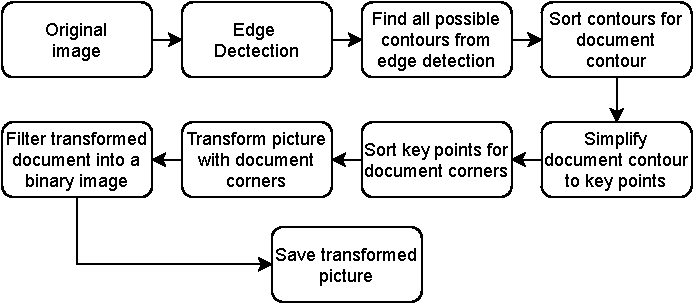
\includegraphics[width=.7\textwidth]{images/pipeline.pdf}
    \caption{Pipeline}
    \label{fig:pipeline}
\end{figure}

This pipeline will be illustrated on the basis of figure \ref{fig:doc_og} which contains a photograph of a folded document.

\begin{figure}[H]
    \centering
    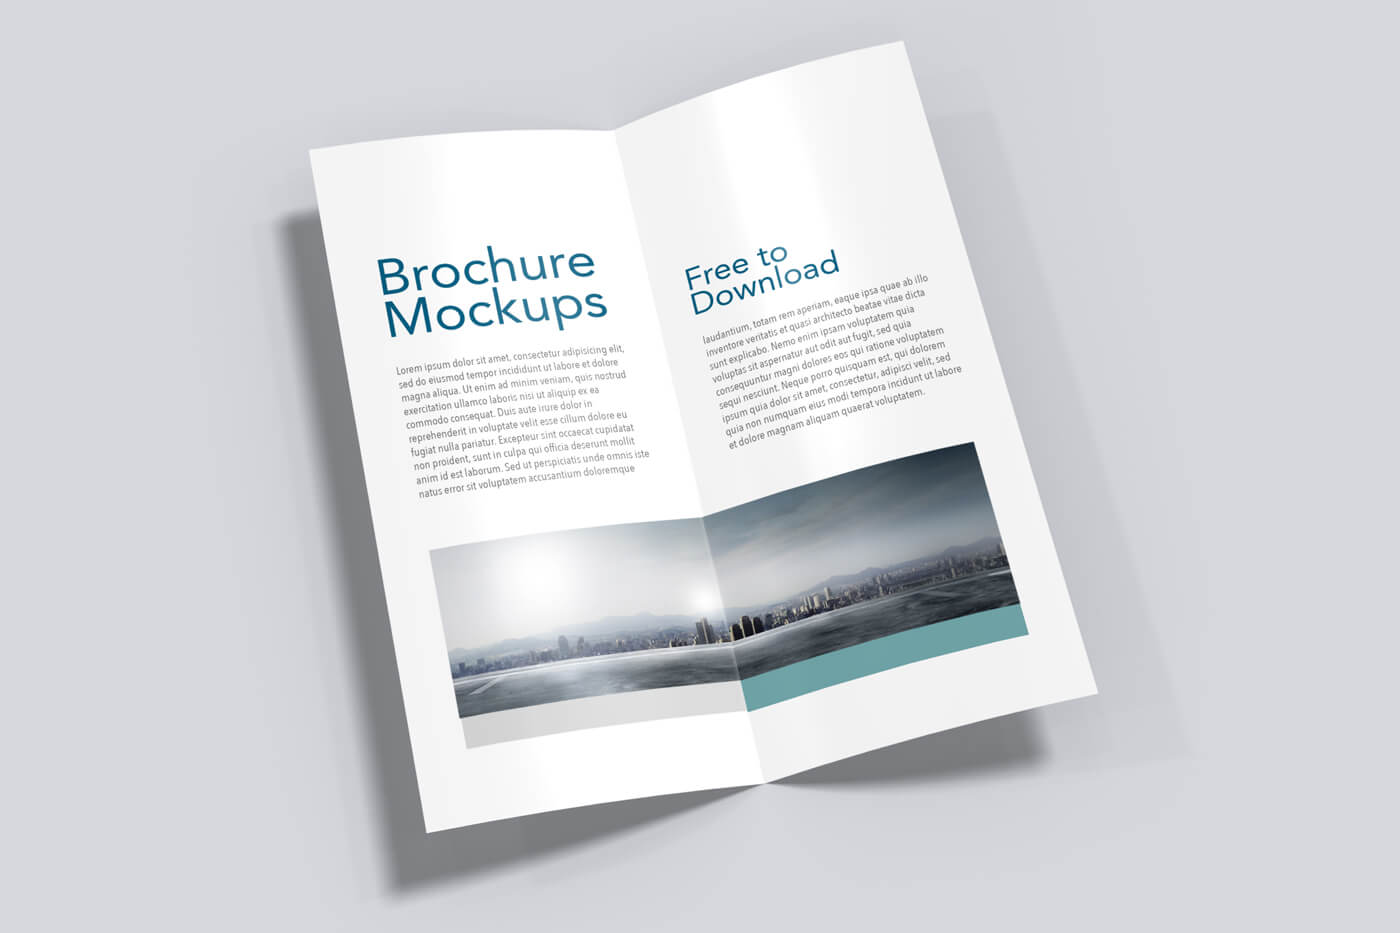
\includegraphics[width=.6\textwidth]{images/3_folded_doc/Brochure-Mockup.jpg}
    \caption{Example image of a photographed Document\\Source: \cite{folded_doc}}
    \label{fig:doc_og}
\end{figure}

The first step is to find all edges in the image. The Canny Edge Detection Algorithm is used for this purpose.

\newpage

\subsection{Canny Edge Detector and Contours}

For the Canny Edge Detector the original image needs to be prepared. For that reason the original image is firstly converted into a grayscale image which is further blurred with a Gaussian filter to reduce noise which the Canny edge detector is sensitive to. After that the edge gradient and direction of every pixel of the blurred image gets filtered out. This gradients undergo further a hysteresis thresholding filtering which decides with a minimal and a maximal threshold which edges are sorted out. \cite{gonzalez} \cite{canny} The result can be seen in figure \ref{fig:doc_edge}.

\begin{figure}[H]
     \centering
     \captionsetup{justification=centering}
     \begin{minipage}[b]{0.5\textwidth}
         \centering
         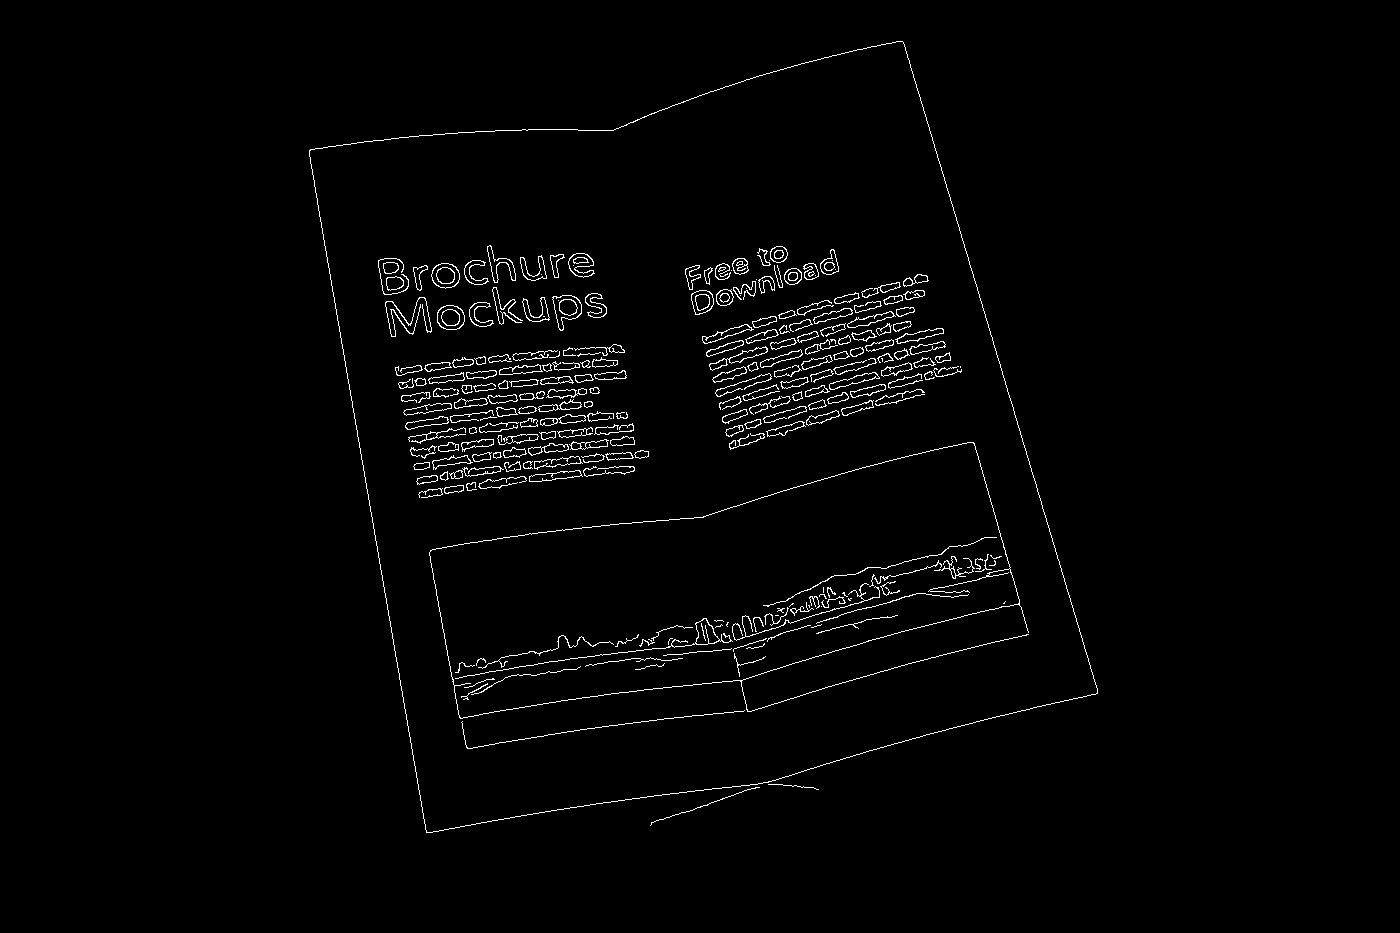
\includegraphics[width=.95\textwidth]{images/3_folded_doc/edged.png}
        \caption{All edges found in the image}
        \label{fig:doc_edge}
     \end{minipage}%
     \begin{minipage}[b]{0.5\textwidth}
         \centering
         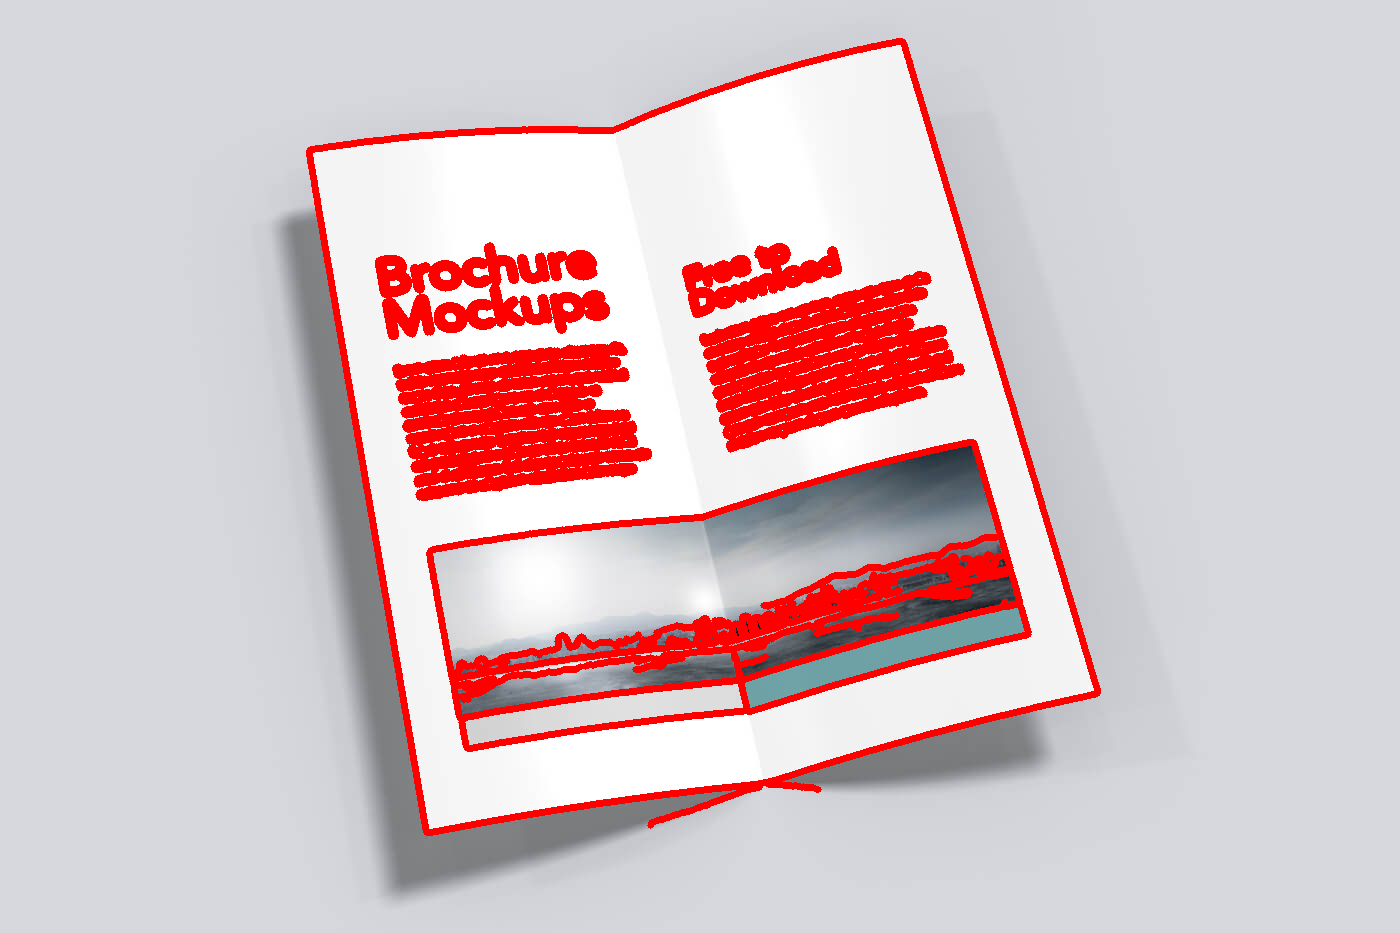
\includegraphics[width=.95\textwidth]{images/3_folded_doc/all_contours.png}
        \caption{All contours found in the image}
        \label{fig:doc_contour}
     \end{minipage}
\end{figure}

\vspace{-3mm}
It can be noted that in figure \ref{fig:doc_edge} not only the document edges are detected. The elements on the document itself and a little bit of the shadow of the document got detected as well. This is important to note in the next steps.\\

The obtained edge data can be turned into contour data. This gives us the advantage of establishing a relationship between the found edge points which can be further classified and examined.\\

A contour "is a list of points that represent, in one way or another, a curve in an image." \cite{oreily} They can also be called a chain of points. Contours join all continuous points into a curve having the same colour or intensity. Therefore we use the binary Canny edge output for this operation. \cite{oreily} \cite{contour}\\

This step would detect all contours in the image like one can see in figure \ref{fig:doc_contour}. Not all of this contours are the searched for document contour. For this we need an algorithm that specifically picks out the document contour.\\

%\newpage

\subsection{Sorting contours and search for the corner points}

That means a sorting algorithm is needed which is used to pick out the longest continuous contour from all available contours. The longest contour is searched for because with the assumptions made, the contour of the document should be the longest continuous line on the image. \\

In comparison to calculating and sorting the contours accordingly to the largest enclosed area of a contour the above mentioned method is preferred because found contours do not have to be closed contours and, consequently, closed areas. \\
Depending on the background lightning, smoothness of the edges of the document, etc. in the image the found contours are not necessarily continuous which is necessary to calculate the enclosed area of the contour.\\

After the longest contour has been found, which can be seen in figure \ref{fig:doc_contour} in red, the contour data can be simplified more to find the key points of our contour: the corner points of the document. Because of our assumptions made, the Ramer–Douglas–Peucker algorithm can be used to reduce the contour data to the searched for corner points.\\ 

The Ramer–Douglas–Peucker algorithm assumes that lines or curves are usually displayed with significantly more points than required. It then tries to find the most significant points in the curve that still describes it approximately. \cite{rdp-algo}\\

It does that by firstly connecting two end points of a curve segment with a straight line with a tolerance band around the line, which is defined by the so called accuracy parameter {\large $\bm{\epsilon}$}. It then checks if the points between the end points are contained in the segment. If they are, they are removed from the list. If they are not, the curve is split up further and the same thinking is applied again on this sub-curve segment. \cite{contour} \cite{rdp-algo}\\

Depending on the accuracy parameter, the total number of points that describes the curve can be significantly reduced. \cite{rdp-algo} In figure \ref{fig:doc_contour} the algorithm could reduce the contour with a total number of 1128 points to exactly 4 points which coincide with the corners of the document.\\

%\newpage

This result can be seen in blue in figure \ref{fig:doc_approx}. In the figure it can be noted that some key points, the folds of the document and shadow contour, got smoothed out in comparison to figure \ref{fig:doc_contour} where these elements are present.

\begin{figure}[H]
     \centering
     \captionsetup{justification=centering}
     \begin{minipage}[t]{0.5\textwidth}
        \centering
        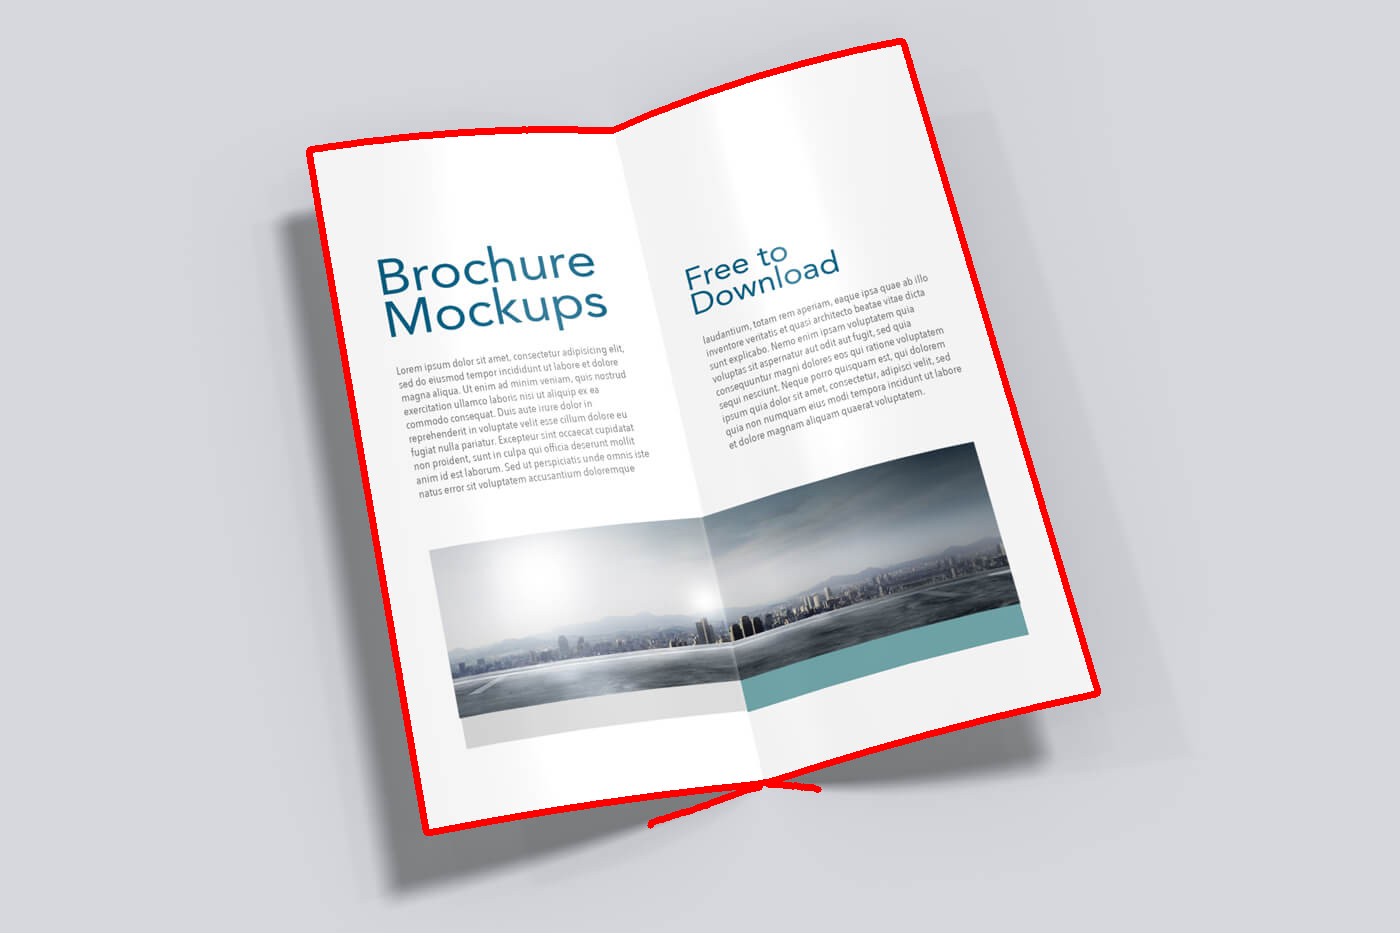
\includegraphics[width=.95\textwidth]{images/3_folded_doc/contours.png}
        \caption{Biggest contour found in the \\image}
        \label{fig:doc_approx}
     \end{minipage}%
     \begin{minipage}[t]{0.5\textwidth}
         \centering
         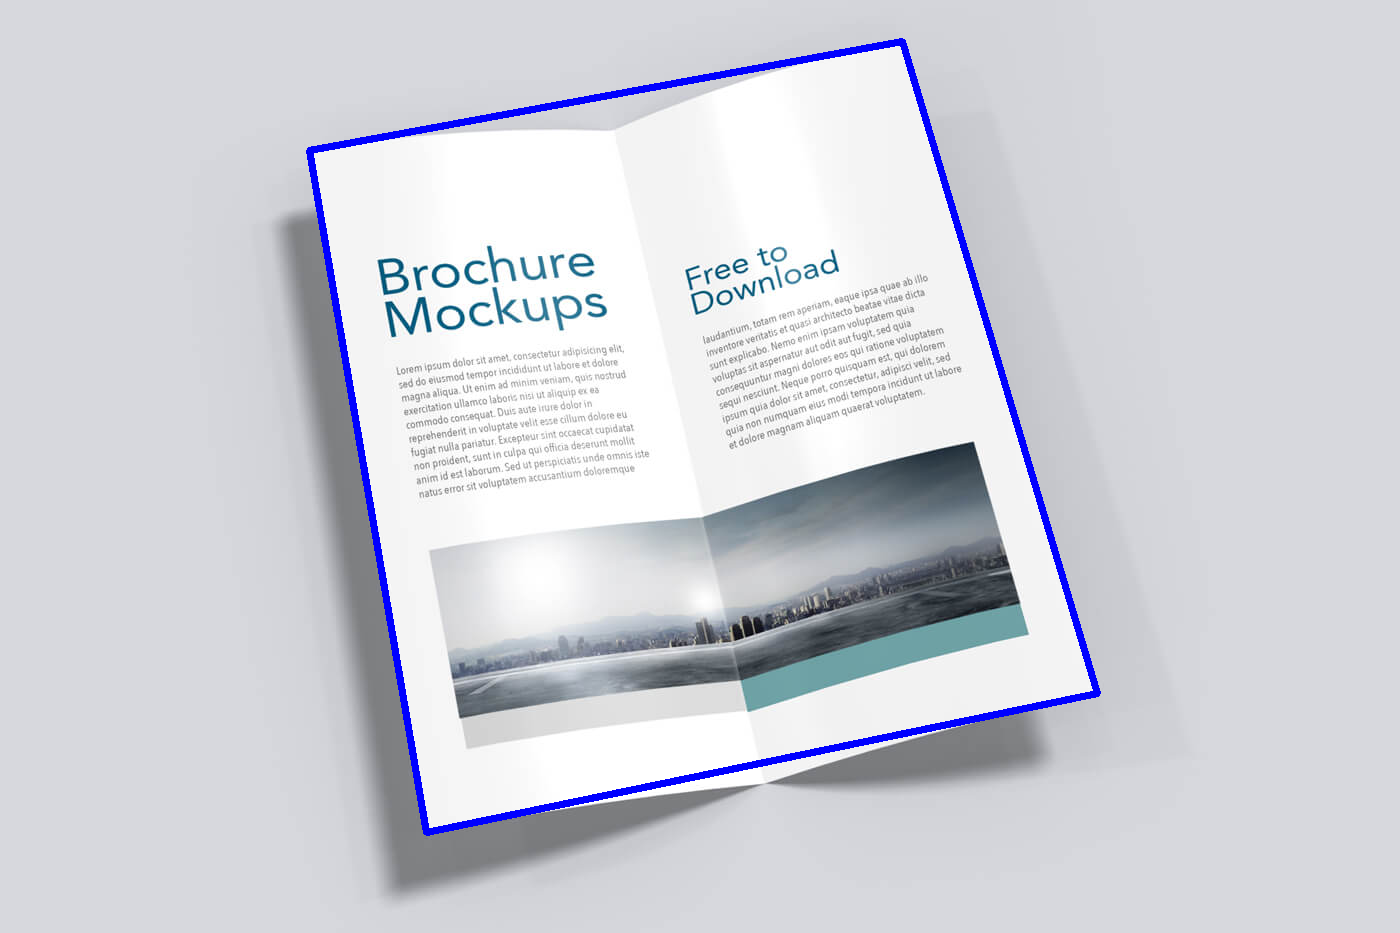
\includegraphics[width=.95\textwidth]{images/3_folded_doc/contours_approx.png}
         \caption{Contour approximation of the \\biggest found contour}
        \label{fig:doc_found_all_corn}
     \end{minipage}
\end{figure}



From the approximation in figure \ref{fig:doc_found_all_corn} the corner points can be easily extracted. However this does not always have to be the case because the number of key points does not always have to be exactly four after the Ramer–Douglas–Peucker algorithm is applied. Especially when the paper is crumpled, more possible key point candidates remain that have to be sorted. \\

For this reason another algorithm is needed that will pick out the corner points from the contour approximation list. In the case we have less than four key points it will be assumed that the image has been insufficiently photographed or an error has occurred because the assumption was made that documents get photographed with at least four key points aka. the corner points.\\

In figure \ref{fig:corner_blank} the bare document model can be seen with the key points P1 to P6. Four of these key points are corner points, seen in green, and two are additional key points which were detected, in purple. \\

\newpage

From the assumption that the document is tilted it can be noted that the corner points are the four most furthest points from all key points in the image. With this in mind we can sort our key point list two times accordingly to the y-axis and the x-axis of the image and pick out the smallest and the biggest entry respectively in this sorted list. This idea can be seen in figure \ref{fig:corner_finder}.\\ 

\vspace{-3mm}

\begin{figure}[H]
    \centering
     \captionsetup{justification=centering}
     \begin{minipage}[t]{0.49\textwidth}
        \centering
        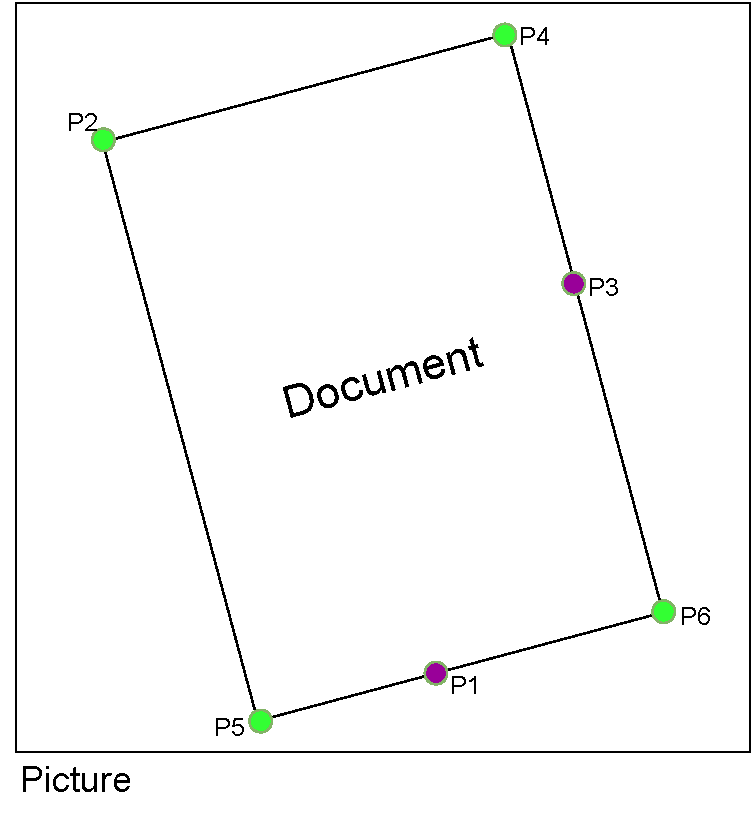
\includegraphics[width=.835\textwidth]{images/custom_figures/corner_finder_blank.pdf}
        \caption{Model of a bare document with key points}
        \label{fig:corner_blank}
     \end{minipage}%
     \begin{minipage}[t]{0.49\textwidth}
        \centering
        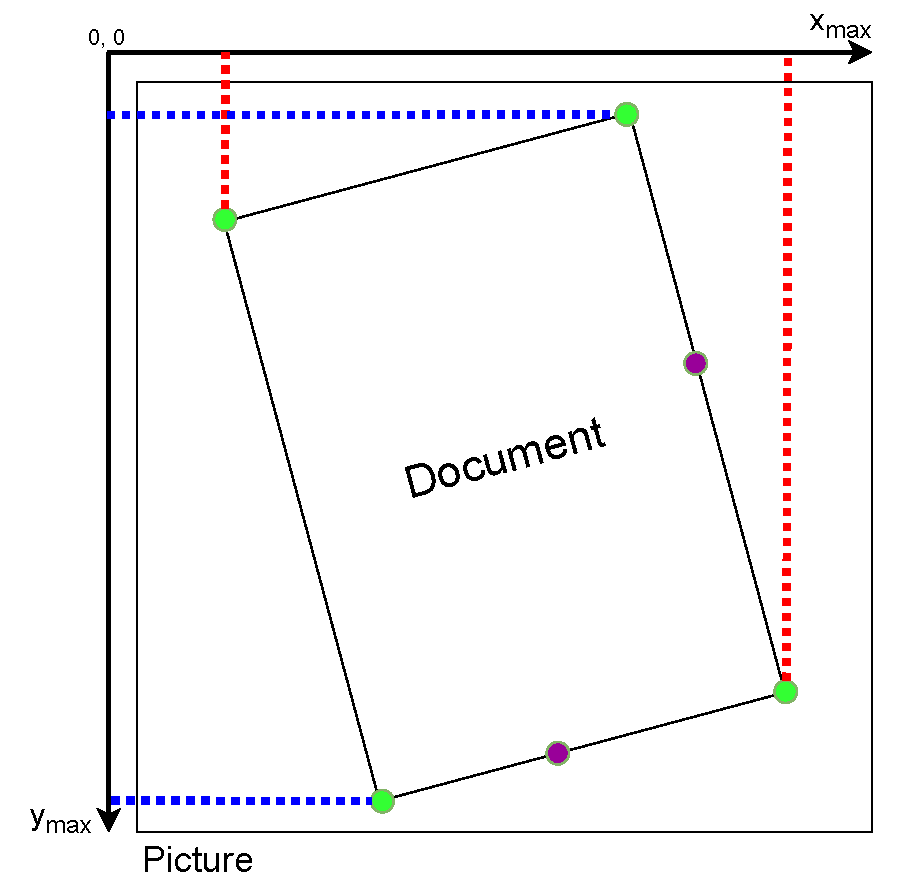
\includegraphics[width=\textwidth]{images/custom_figures/corner_finder_idea.pdf}
        \caption{Diagram of the corner finder Algorithm}
        \label{fig:corner_finder}
     \end{minipage}
\end{figure}

The drawback is that if the document is photographed exactly perpendicular to the axis then the corner points are exactly on the same y-axis and the x-axis with another corner point. Therefore it is not ensured that the first and last are the searched for corner points.\\

Another possibility to search for the corner points in the key points list would be to add or subtract the x- and y-coordinates for every entry in the list. Since the corner points are the furthest points in the image, they can also be set in relation to their x- and y-coordinates. For example is the key point P6 the biggest sum of his coordinates from all entries in the key point list.\\

However this method is not used here because in the edge case that two key points have the same result, in addition or subtraction, it is unclear which one of them is the corner point. If no catch mechanism has been implemented for this edge case, the entire application crashes. With the other method the completion of the application would be possible.\\

\subsection{Perspective Transformation and binary image}

Finally with the four found corner points of the document it can now be subjected to a perspective transformation. For this, the height and width of the document must be calculated to form the transformation matrix with which we can transform our image. To calculate the transformation matrix, destination height and width is needed which is our document height and width.\\ 

To calculate the width and height of document we can use the bare document model in figure \ref{fig:corner_blank}. Since the four corner points have been determined we can compute the distance between them with the Pythagorean theorem. \\

\begin{wrapfigure}{R}{0.45\textwidth}
    \centering
    \captionsetup{justification=centering}
    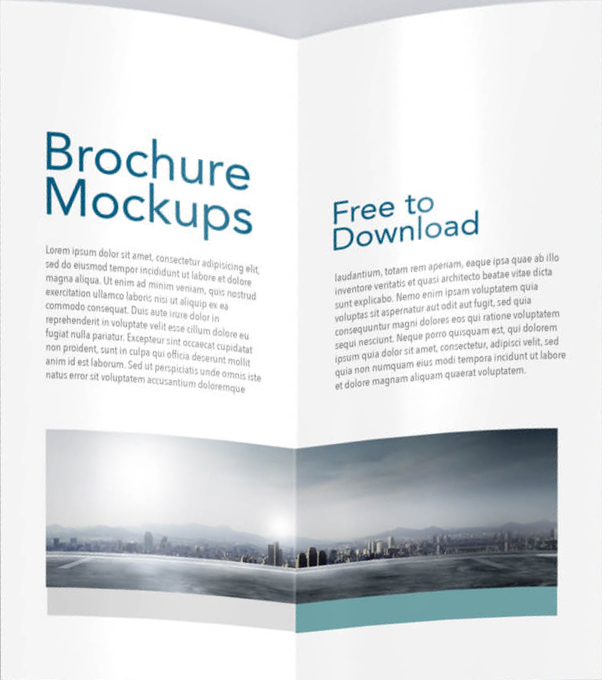
\includegraphics[width=.4\textwidth]{images/3_folded_doc/warped.png}
    \caption{Perspective transformed document}
    \label{fig:doc_warped}
    \vspace{-5mm}
\end{wrapfigure}

Since it can be assumed that the camera did not take the image at a right angle to the document, two identical edges of the document do not have to be the same length when they are calculated. That means for example if the document has been photographed from an angle that the right edge height between P4 and P6 does not have to be the same as the left edge height between P2 and P5.\\

This should be in most cases a minimal difference. In this case, the higher value of the two is taken as this ensures that the complete document appears in the final image even if from the background more than necessary was transformed too.\\

After that the perspective transformation can be carried out and the result can be seen in figure \ref{fig:doc_warped}. As could already be guessed from figure \ref{fig:doc_found_all_corn}, a part of the document has been cut off and a part of the background got transformed too. \\
 
\newpage
 
This is due to the assumption that a document has only four corner points. The document shown here could still be transformed with the assumptions made but not to the extent that only all of the document is visible. For this a more sophisticated approach is needed.\\ 

\begin{wrapfigure}{R}{0.45\textwidth}
    \centering
    \captionsetup{justification=centering}
    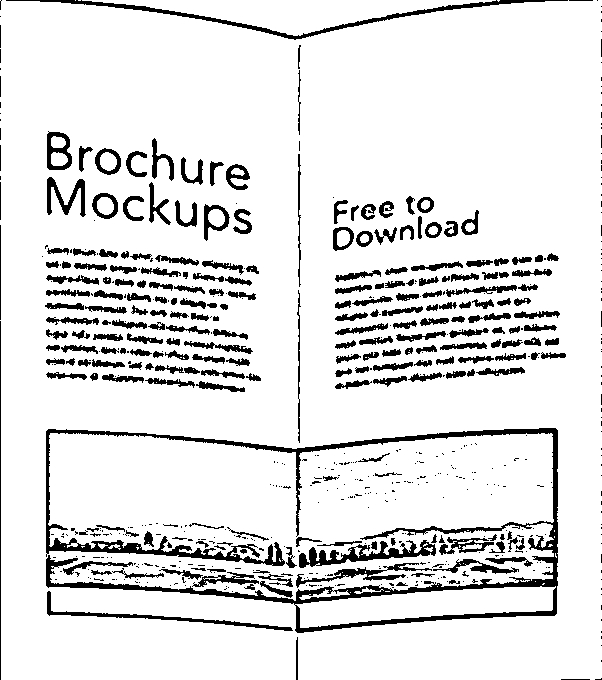
\includegraphics[width=.4\textwidth]{images/3_folded_doc/result.jpg}
    \caption{Binary image with adaptive thresholding}
    \label{fig:doc_binary}
    \vspace{-2mm}
\end{wrapfigure}


Now the transformed image only has to be saved. For that the picture needs to be converted into a binary image. Given that documents are being photographed under real world lightning conditions, an adaptive thresholding technique will be used. \cite{threshold} These conditions can be seen very well in figure \ref{fig:doc_warped}.\\

For the adaptive thresholding technique the transformed image needs to be prepared. For that reason the transformed image is converted first into a grayscale image which is further blurred with a Gaussian filter. Afterwards for every pixel a weighted average gets calculated with a kernel of the size $k\times k$. That means that every pixel has its own threshold value with which it gets classified. If the pixel is smaller than his calculated threshold it is set to 0, otherwise it is set to 255. Optionally for every threshold a constant \textbf{C} can be subtracted. \cite{oreily} \cite{threshold} The result can be seen in figure \ref{fig:doc_binary}.\\

As can be seen from the figure \ref{fig:doc_binary} the used technique or parameters do not fit perfectly for this image because the smaller text in the document is not as readable as the big letters or the image beneath the text. In general though the technique is a good approach for documents because documents do not have in general sharply changing lightning conditions such as for example reflective objects .
\section{Testing the Implementation}

To test the implementation of the presented document scanner for faults, a variety of test images are needed. For that the sample images from the \textit{OpenCV-Document-Scanner} Project [\url{https://github.com/andrewdcampbell/OpenCV-Document-Scanner}] are used.\\
In this chapter however only the flawed images will be examined in more detail, as they better illustrate the flaws in our implementation.\\

The following parameters are used after extended testing on the test images:
\begin{enumerate}
    \item \textbf{Canny Edge Detector}:\\
    Used was a Gaussian filter with a kernel of size 7x7 and a Canny Edge Detector Algorithm with a minimum threshold of 0 and a maximum threshold of 84.
    \item \textbf{Ramer–Douglas–Peucker algorithm}:\\
    Used was an accuracy parameter {\large $\bm{\epsilon}$} of 5 percent.
    \item \textbf{Adaptive Thresholding}:\\
    Used was a Gaussian filter with a kernel of size 5x5 to smooth the image. For the adaptive threshold technique a Gaussian Kernel of size $11 \times 11$ and a constant \textbf{C} of 2 were used.
\end{enumerate}

At the end of the test procedure one of the images which still got transformed incorrectly was the image \textit{notepad.jpg} from the \textit{OpenCV-Document-Scanner} Project seen in figure \ref{fig:note_error}.

\begin{figure}[H]
     \centering
     \captionsetup{justification=centering}
     \begin{subfigure}[t]{0.3\textwidth}
         \centering
         
\includegraphics[width=\textwidth]{images/4_image/notepad.png}
         \caption{Original image}
         \label{fig:note_og}
     \end{subfigure}
     \hfill
     \begin{subfigure}[t]{0.3\textwidth}
         \centering
         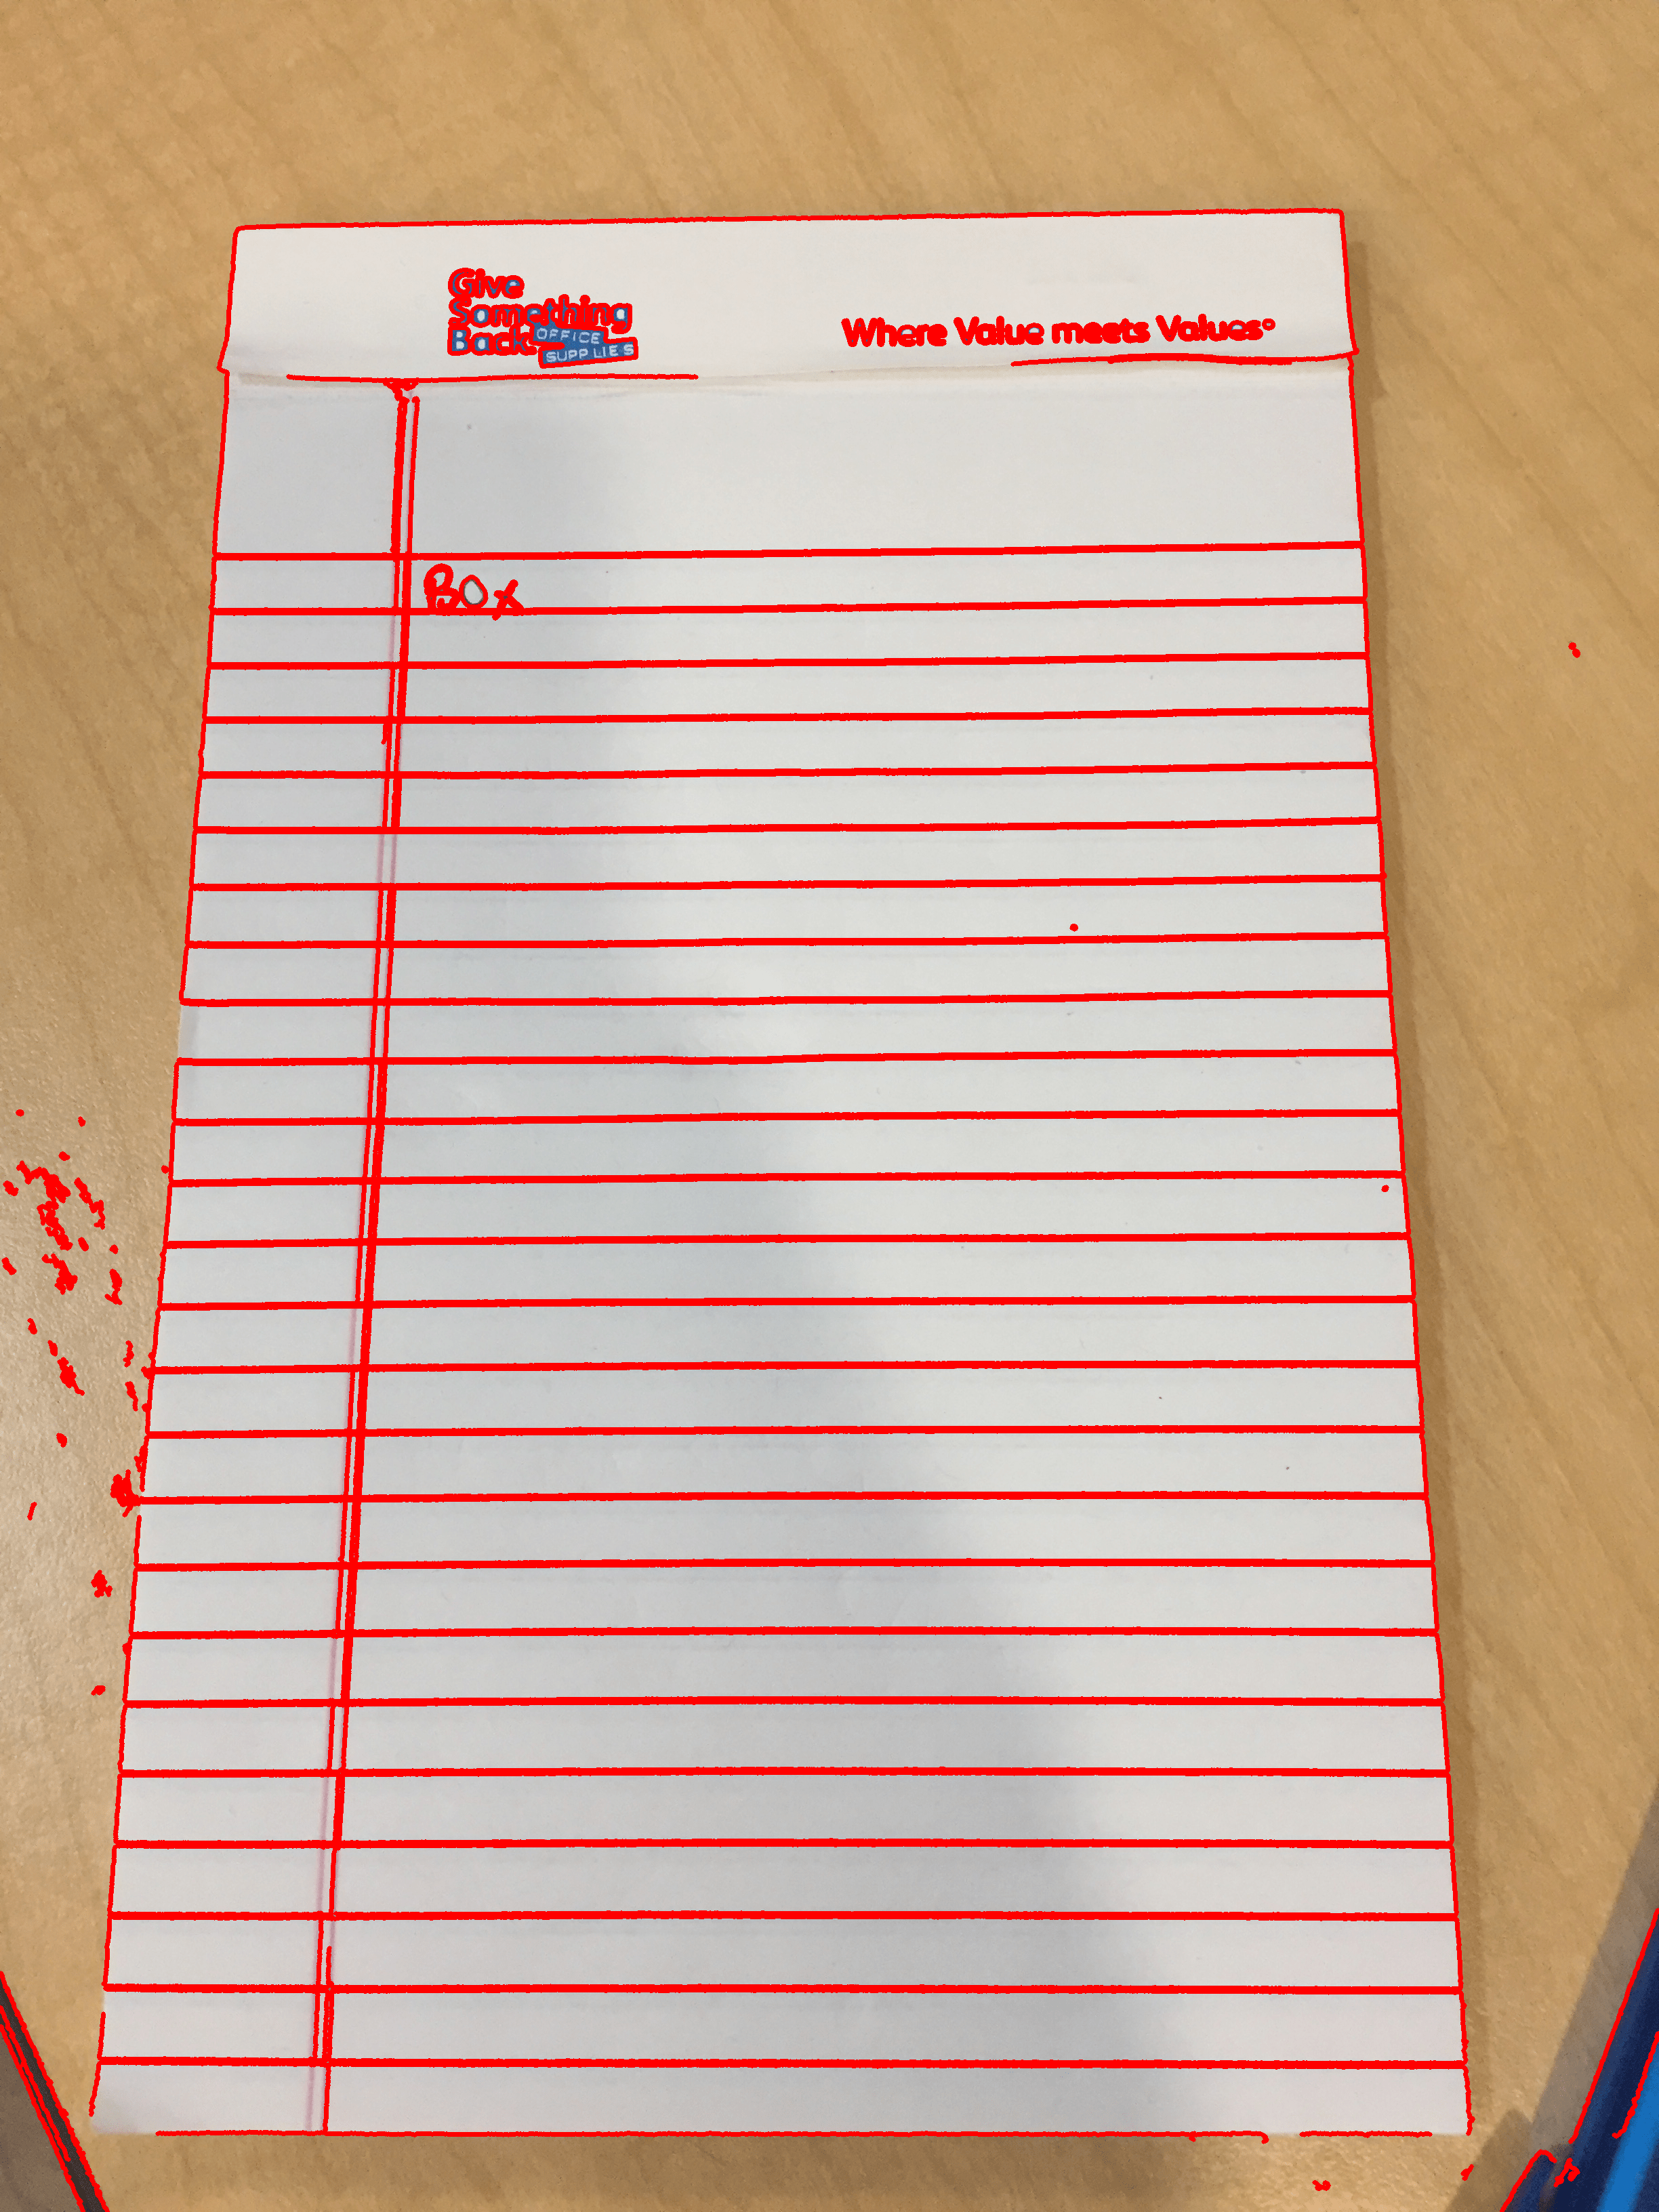
\includegraphics[width=\textwidth]{images/4_image/contours.png}
         \caption{All contours found in image}
         \label{fig:note_all}
     \end{subfigure}
     \hfill
     \begin{subfigure}[t]{0.3\textwidth}
         \centering
         
\includegraphics[width=\textwidth]{images/4_image/biggest_contour.png}
         \caption{Biggest found contour in image}
         \label{fig:note_biggest}
     \end{subfigure}
        \caption{Incorrectly transformed image of a document}
        \label{fig:note_error}
\end{figure}

\newpage

In figure \ref{fig:note_biggest} the problem can be seen clearly: The longest contour found from all possible contours is not the document edge. The problem occurs because the document edges are connected to contours inside the document, which artificially creates a longer contour that does not have to include all document corner points.\\

This is a weak point of this implementation. If there is a document that contains elements within the document which intersect the document edge, there is a chance that the longest found contour is not the document edge. Therefore the document corner points cannot be determined correctly.\\

A solution to this problem would be to let the user manually decide where to place the corner points if he is unsatisfied with the results. This could be for example if he feels that the corner points are not placed exactly on the corners of the document or if even no corner points have been detected. This is the same approach as the \textit{OpenCV-Document-Scanner} Project uses.


\sloppy %Latex soll nicht so viel Sand in der Vagina haben
\printbibliography[heading=bibintoc] % , title={Literaturverzeichnis}
\fussy  %Latex soll wieder genau soviel Sand in der Vagina haben

\end{document}
